\documentclass[aspectratio=169,10pt]{beamer}

\usetheme{metropolis}
\usepackage{appendixnumberbeamer}
\usepackage{booktabs}
\usepackage[scale=2]{ccicons}
\usepackage{pgfplots}
\usepgfplotslibrary{dateplot}
\usepackage{xspace}
\usepackage{tikz}
\usetikzlibrary{mindmap,trees,shapes,arrows,positioning}
\usepackage{tcolorbox}

\title{Navigating Your Computer Science PhD Journey in Germany}
\subtitle{Session 2: Financial Planning, Practical Considerations, and Career Development}
\date{\today}
\author{Dr. [Your Name]}
\institute{[Your Institution]}

\begin{document}

\maketitle

\begin{frame}{Recap and Today's Agenda}
\begin{columns}[T]
    \begin{column}{0.5\textwidth}
        \alert{Recap from Talk 1}
        \begin{itemize}
            \item Overview of CS PhD programs in Germany
            \item Application process and requirements
            \item Finding supervisors and research groups
        \end{itemize}
    \end{column}
    \begin{column}{0.5\textwidth}
        \alert{Today's Agenda}
        \begin{itemize}
            \item Financial planning for your CS PhD
            \item Housing and practical considerations
            \item Visa and legal matters
            \item Navigating German bureaucracy
            \item Work-life balance and cultural integration
            \item Career development for CS PhDs
        \end{itemize}
    \end{column}
\end{columns}
\end{frame}

\begin{frame}{Financial Planning for Your CS PhD}
\begin{itemize}
    \item \textbf{Living Costs Breakdown}
    \begin{itemize}
        \item Rent: €400-€800 (varies by city)
        \item Food: €200-€300
        \item Health Insurance: €110 (approx.)
        \item Public Transportation: €30-€80
    \end{itemize}
    \item \textbf{Research Expenses}
    \begin{itemize}
        \item Conference travel: €1000-€2000 per conference
        \item Equipment: Often provided by the university
    \end{itemize}
    \item \textbf{Tax Implications}
    \begin{itemize}
        \item PhD positions: Taxed as regular income
        \item Scholarships: Often tax-free, but check specific terms
    \end{itemize}
    \item \textbf{Funding Sources}
    \begin{itemize}
        \item University positions (TVL-E13, 50-100%)
        \item DFG grants
        \item Industry collaborations
        \item DAAD scholarships
    \end{itemize}
\end{itemize}
\end{frame}

\begin{frame}{Housing and Practical Considerations}
\begin{itemize}
    \item \textbf{Finding Accommodation}
    \begin{itemize}
        \item University housing offices
        \item WG-Gesucht.de, Immobilienscout24.de
        \item Facebook groups for housing
    \end{itemize}
    \item \textbf{Rental Contracts}
    \begin{itemize}
        \item Understand "warm" vs. "cold" rent
        \item Security deposit (usually 2-3 months' rent)
        \item Notice periods for moving out
    \end{itemize}
    \item \textbf{Setting Up Utilities}
    \begin{itemize}
        \item Internet providers: Telekom, Vodafone, O2
        \item Electricity: Check for best rates on Verivox.de
    \end{itemize}
    \item \textbf{Healthcare System}
    \begin{itemize}
        \item Public vs. Private insurance
        \item Finding English-speaking doctors
    \end{itemize}
\end{itemize}
\end{frame}

\begin{frame}{Visa and Legal Considerations}
\begin{itemize}
    \item \textbf{Visa Requirements (Non-EU)}
    \begin{itemize}
        \item Student visa for PhD studies
        \item Documents: Admission letter, proof of funding, health insurance
    \end{itemize}
    \item \textbf{Registration and Permits}
    \begin{itemize}
        \item City registration (Anmeldung) within 2 weeks of arrival
        \item Residence permit application
    \end{itemize}
    \item \textbf{Working Regulations}
    \begin{itemize}
        \item 120 full days or 240 half days per year allowed
        \item No limit if work is related to research
    \end{itemize}
    \item \textbf{Long-term Prospects}
    \begin{itemize}
        \item EU Blue Card eligibility after graduation
        \item Permanent residency options
    \end{itemize}
\end{itemize}
\end{frame}

\begin{frame}{Navigating German Bureaucracy}
\begin{itemize}
    \item \textbf{Key Administrative Tasks}
    \begin{itemize}
        \item City registration (Anmeldung)
        \item Opening a bank account
        \item Health insurance registration
    \end{itemize}
    \item \textbf{Dealing with Authorities}
    \begin{itemize}
        \item Ausländerbehörde (Foreigners' Office)
        \item Bürgeramt (Citizens' Office)
    \end{itemize}
    \item \textbf{Resources and Support}
    \begin{itemize}
        \item University International Office
        \item Welcome Centers in major cities
        \item Online platforms: Make it in Germany, Study in Germany
    \end{itemize}
    \item \textbf{Tips}
    \begin{itemize}
        \item Prepare documents in advance
        \item Learn basic German phrases
        \item Be patient and persistent
    \end{itemize}
\end{itemize}
\end{frame}

\begin{frame}{Work-Life Balance and Cultural Integration}
\begin{itemize}
    \item \textbf{Managing Workload}
    \begin{itemize}
        \item Set realistic goals and timelines
        \item Use productivity techniques (e.g., Pomodoro)
        \item Regular check-ins with supervisor
    \end{itemize}
    \item \textbf{Leisure and Social Life}
    \begin{itemize}
        \item Join university sports groups
        \item Attend local tech meetups and hackathons
        \item Explore German cuisine and traditions
    \end{itemize}
    \item \textbf{Language Learning}
    \begin{itemize}
        \item University language courses
        \item Tandem language exchange
        \item Online resources: Duolingo, Deutsche Welle
    \end{itemize}
    \item \textbf{Cultural Adaptation}
    \begin{itemize}
        \item Understand German academic culture
        \item Respect for punctuality and direct communication
        \item Embrace "Feierabend" culture (work-life separation)
    \end{itemize}
\end{itemize}
\end{frame}

\begin{frame}{Overcoming Common Challenges in CS PhDs}
\begin{itemize}
    \item \textbf{Imposter Syndrome}
    \begin{itemize}
        \item Recognize it's common in tech fields
        \item Focus on growth and learning, not comparison
        \item Celebrate small wins and milestones
    \end{itemize}
    \item \textbf{Research Setbacks}
    \begin{itemize}
        \item View failures as learning opportunities
        \item Seek advice from peers and mentors
        \item Break complex problems into smaller tasks
    \end{itemize}
    \item \textbf{Supervisor Relationships}
    \begin{itemize}
        \item Establish clear expectations early
        \item Regular communication and progress reports
        \item Be proactive in seeking feedback
    \end{itemize}
    \item \textbf{Balancing Responsibilities}
    \begin{itemize}
        \item Prioritize tasks effectively
        \item Learn to say no to non-essential commitments
        \item Use time management tools (e.g., Trello, Asana)
    \end{itemize}
\end{itemize}
\end{frame}

\begin{frame}{Career Development for CS PhD Students}
\begin{itemize}
    \item \textbf{Skill Development}
    \begin{itemize}
        \item Software engineering best practices
        \item Data science and machine learning techniques
        \item Project management and team leadership
    \end{itemize}
    \item \textbf{Internship Opportunities}
    \begin{itemize}
        \item Research internships at tech giants (Google, Microsoft, etc.)
        \item Collaboration with local tech startups
        \item Academic visits to other institutions
    \end{itemize}
    \item \textbf{Teaching and Mentoring}
    \begin{itemize}
        \item TA positions for CS courses
        \item Supervising Bachelor's or Master's theses
        \item Organizing coding workshops or hackathons
    \end{itemize}
    \item \textbf{Career Preparation}
    \begin{itemize}
        \item Build a strong GitHub portfolio
        \item Contribute to open-source projects
        \item Network at conferences and tech events
        \item Explore both academic and industry options
    \end{itemize}
\end{itemize}
\end{frame}

\begin{frame}{Publishing and Conferences in CS}
\begin{itemize}
    \item \textbf{Publishing Strategies}
    \begin{itemize}
        \item Focus on top-tier conferences (e.g., ICSE, SIGCOMM, NeurIPS)
        \item Balance between conferences and journals
        \item Consider workshops for early-stage ideas
    \end{itemize}
    \item \textbf{Effective Presentations}
    \begin{itemize}
        \item Practice your talks extensively
        \item Use clear, visually appealing slides
        \item Prepare for Q\&A sessions
    \end{itemize}
    \item \textbf{Open Science Practices}
    \begin{itemize}
        \item Share code on GitHub or GitLab
        \item Use preprint servers (e.g., arXiv)
        \item Consider open-access publishing options
    \end{itemize}
    \item \textbf{Networking at Conferences}
    \begin{itemize}
        \item Prepare an "elevator pitch" for your research
        \item Attend social events and poster sessions
        \item Follow up with new contacts after the conference
    \end{itemize}
\end{itemize}
\end{frame}

\begin{frame}{Mental Health and Support Systems}
\begin{itemize}
    \item \textbf{Recognizing Stress and Burnout}
    \begin{itemize}
        \item Watch for signs: exhaustion, cynicism, reduced productivity
        \item Take regular breaks and vacations
        \item Practice self-care and mindfulness
    \end{itemize}
    \item \textbf{University Services}
    \begin{itemize}
        \item Counseling centers with English-speaking therapists
        \item Workshops on stress management and mental health
        \item Sports and fitness facilities for stress relief
    \end{itemize}
    \item \textbf{Peer Support}
    \begin{itemize}
        \item Join or create PhD support groups
        \item Participate in mentoring programs
        \item Share experiences with fellow international students
    \end{itemize}
    \item \textbf{Work-Life Balance}
    \begin{itemize}
        \item Set boundaries between work and personal time
        \item Pursue hobbies and interests outside of CS
        \item Build a social network beyond your research group
    \end{itemize}
\end{itemize}
\end{frame}

\begin{frame}{Looking Ahead: Post-PhD Opportunities}
\begin{itemize}
    \item \textbf{Academic Careers}
    \begin{itemize}
        \item Postdoc positions in Germany or abroad
        \item Junior professorships and tenure-track options
        \item Research scientist roles at institutions
    \end{itemize}
    \item \textbf{Industry Opportunities}
    \begin{itemize}
        \item R\&D positions in tech companies
        \item Data scientist and machine learning engineer roles
        \item Software architect and tech lead positions
    \end{itemize}
    \item \textbf{Entrepreneurship}
    \begin{itemize}
        \item Tech startup ecosystems in Berlin, Munich, Hamburg
        \item University spin-off support programs
        \item Accelerators and incubators for deep tech
    \end{itemize}
    \item \textbf{Research Labs}
    \begin{itemize}
        \item Industrial research labs (e.g., IBM Research, Microsoft Research)
        \item Government research institutions (e.g., Fraunhofer, Max Planck)
        \item Cross-disciplinary research centers
    \end{itemize}
\end{itemize}
\end{frame}

\begin{frame}{Q\&A Session}
\centering
\large{Time for Your Questions!}

\vspace{1cm}

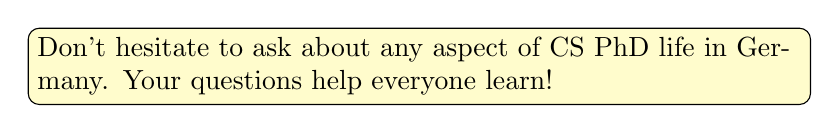
\begin{tikzpicture}
    \node[draw,rounded corners,fill=yellow!20,text width=0.8\textwidth] {
        Don't hesitate to ask about any aspect of CS PhD life in Germany. Your questions help everyone learn!
    };
\end{tikzpicture}
\end{frame}

\begin{frame}{Conclusion and Next Steps}
\begin{itemize}
    \item \textbf{Key Takeaways}
    \begin{itemize}
        \item Plan your finances carefully
        \item Embrace the challenges of living and studying in Germany
        \item Focus on both research excellence and broader skill development
        \item Take care of your mental health and work-life balance
        \item Start planning your post-PhD career early
    \end{itemize}
    \item \textbf{Next Steps}
    \begin{itemize}
        \item Create a budget plan for your PhD years
        \item Start or improve your German language learning
        \item Set specific research and personal development goals
        \item Explore potential conferences and publication venues
        \item Connect with current CS PhD students for more insights
    \end{itemize}
\end{itemize}

\vspace{0.5cm}
\centering
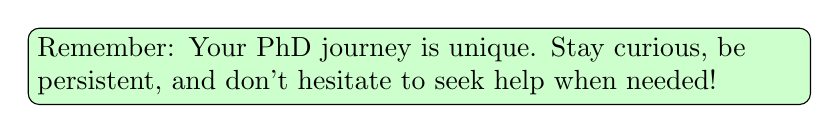
\begin{tikzpicture}
    \node[draw,rounded corners,fill=green!20,text width=0.8\textwidth] {
        Remember: Your PhD journey is unique. Stay curious, be persistent, and don't hesitate to seek help when needed!
    };
\end{tikzpicture}
\end{frame}

\end{document}